\chapter{Metodologías de Desarrollo de Software}
\label{cp:software-methodology}

\parindent0pt

En el ámbito del desarrollo de software, la selección de una metodología de trabajo adecuada es un factor determinante para garantizar la eficacia y el éxito de un proyecto. La planificación y ejecución de este trabajo de tesis depende en gran medida de la estructura metodológica que se elija. La selección de una metodología es necesaria considerando que las metodologías no son soluciones universales, sino herramientas que deben ajustarse a las necesidades específicas de cada proyecto, tomando en cuenta aspectos como los objetivos, el alcance, el equipo involucrado y la forma de entrega de los resultados.

El objetivo principal de esta sección es realizar un análisis detallado de las principales metodologías de desarrollo de software conocidas, evaluando sus características y su aplicabilidad en función de los requerimientos y condiciones particulares del trabajo de tesis. Para ello, se han considerado tanto metodologías tradicionales como ágiles, cada una con enfoques y principios diferentes, pero con un mismo fin: facilitar el desarrollo de un software funcional que cumpla con los objetivos planteados en este proyecto.

A lo largo de este análisis, se compararán metodologías clave en función de varios criterios, como la definición de requerimientos, la planificación de actividades, y la flexibilidad frente a cambios. Este enfoque permitirá identificar la metodología más adecuada que permita no solo el cumplimiento de los plazos y los objetivos técnicos, sino también una integración fluida de los distintos aspectos del desarrollo y la entrega final del software.

Con el objetivo de elegir la metodología de trabajo más adecuada para el desarrollo de software de este trabajo de tesis, se analizaron varias metodologías distintas teniendo en cuenta los siguientes aspectos:

\begin{itemize}
    \item Objetivos del trabajo de tesis
    \item Planificación de actividades
    \item Alcance del prototipo
    \item Definición de requerimientos funcionales y no funcionales
    \item Modalidad de entrega de resultados
    \item Equipo de trabajo
\end{itemize}

Se analizaron diferentes metodologías de trabajo para el desarrollo de software, incluyendo metodologías de trabajo tradicionales y metodologías ágiles para determinar cuál se ajusta mejor a este proyecto. Tras la revisión general de metodologías existentes, comparamos en distintos aspectos claves con produndidad un grupo selecto de 5 metodologías que consideramos más adecuadas para el desarrollo de software de este trabajo de tesis tras el análisis previo. 

\section{Metodologías de desarrollo de software}

Las metodologías de desarrollo de software pueden clasificarse en dos grandes categorías: prescriptivas y evolutivas. Los modelos prescriptivos o tradicionales, ofrecen una estructura y un orden definidos, orientados a maximizar la previsibilidad y la eficiencia en entornos bien entendidos y con pocos cambios. Estos modelos tradicionales introdujeron disciplina en la práctica de la ingeniería de software, aunque su rigidez puede ser una limitante en proyectos donde los requerimientos son inciertos o susceptibles a cambios frecuentes.

Por otro lado, los modelos de proceso evolutivo y el desarrollo ágil se adaptan mejor a las realidades dinámicas del desarrollo de software moderno. Permiten una iteración continua y la adaptación frente a los cambiantes requerimientos del negocio y la tecnología. El desarrollo ágil, en particular, pone énfasis en la flexibilidad, la colaboración continua con el cliente y la capacidad de responder a cambios con rapidez y eficacia. Los enfoques ágiles son valorados por su capacidad de facilitar la entrega rápida de software funcional y adaptarse a las necesidades cambiantes del proyecto y del mercado.

Existen montones de metodologías de desarrollo de software, cada una con sus propias ventajas y desventajas. Para elegir la metodología adecuada para este trabajo, se filtraron y preseleccionaron 5 metodologías de desarrollo de software que se consideraron más adecuadas para el desarrollo de software de este trabajo de tesis. Estas metodologías son:

\begin{itemize}
		\item Modelo en cascada
		\item Modelo en V
		\item Modelo espiral
		\item Metodología Scrum
		\item Metodología Kanban
\end{itemize}

A continuación, se presenta una descripción y un análisis de cada una de estas metodologías, evaluando sus características, ventajas y desventajas, y su aplicabilidad en función de los requerimientos y condiciones particulares del trabajo de tesis.


\subsection{Modelo en cascada}

La metodología en cascada es uno de los enfoques más antiguos y estructurados en el desarrollo de software. Este modelo es secuencial y lineal, lo cual implica que las fases del proyecto deben completarse en un orden específico sin posibilidad de retorno una vez finalizadas. Estas fases incluyen la especificación de requerimientos, planeación, modelado, implementación, despliegue y mantenimiento. Cada una de estas etapas debe ser completada satisfactoriamente antes de avanzar a la siguiente, garantizando así una planificación clara y una estructura bien definida \cite{pressman2010ingeneria}.

\begin{figure}[h]
    \centering
    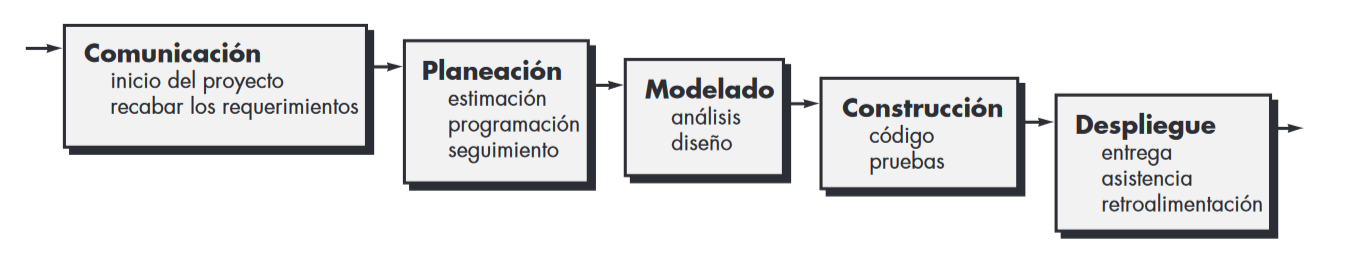
\includegraphics[width=\linewidth]{Figures/model-waterfall.png}
    \caption{Modelo en cascada. Fuente: \cite{pressman2010ingeneria}}
\end{figure}


Este modelo es ideal para proyectos donde los requerimientos son bien conocidos y estables desde el inicio, como en las adaptaciones a sistemas existentes que requieren modificaciones específicas por cambios regulatorios. Sin embargo, este modelo ha sido criticado por su rigidez y por la dificultad que presenta ante la necesidad de adaptarse a cambios durante el desarrollo del software. Problemas como la dificultad de los clientes para expresar todos los requerimientos inicialmente y los riesgos de descubrir errores tardíamente en el proceso son inherentes al modelo en cascada. Estos desafíos pueden llevar a lo que se conoce como "estados de bloqueo", donde la dependencia entre tareas secuenciales causa inactividad y retrasos significativos.

\subsection{Modelo en V}

El modelo en V es una variante del modelo de cascada que añade un enfoque sistemático en la verificación y validación de cada etapa del desarrollo del software \cite{pressman2010ingeneria}. Este modelo sigue un enfoque secuencial, de forma similar al modelo en cascada, sin embargo, se diferencia en que cada fase de desarrollo está emparejada con una fase de prueba correspondiente, formando una estructura en forma de "V". A medida que el proyecto avanza hacia abajo en la primera mitad de la V, los requisitos y componentes del sistema son detallados cada vez más. Una vez completada la codificación, el proceso asciende por el lado derecho de la V, donde cada etapa de desarrollo anterior es validada a través de pruebas detalladas.

\begin{figure}[h]
	\centering
	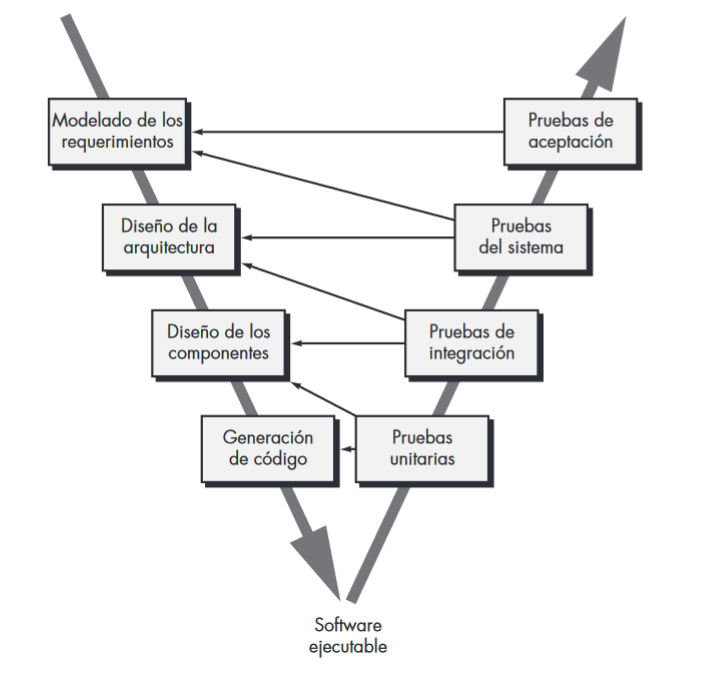
\includegraphics[width=\linewidth]{Figures/model-v.png}
	\caption{Modelo en V. Fuente: \cite{pressman2010ingeneria}}
\end{figure}

Esta metodología es útil para asegurar que cada componente del software sea validado en paralelo a su creación, permitiendo la detección y corrección temprana de errores. Este enfoque ayuda a minimizar los riesgos al final del proyecto, haciendo del modelo en V una opción fuerte para proyectos que requieren altos estándares de calidad y donde los errores tempranos podrían tener consecuencias costosas o críticas. Aunque este modelo comparte algunas limitaciones con el modelo en cascada, como la dificultad para adaptarse a cambios significativos una vez que el proyecto está en curso, su estructura permite una mejor gestión del riesgo y calidad mediante la validación constante de cada etapa del desarrollo.

\subsection{Modelo espiral}

El modelo espiral es un enfoque evolutivo que combina la iteración de los prototipos con la rigurosidad sistemática del modelo en cascada \cite{pressman2010ingeneria}. Este modelo se distingue por su enfoque cíclico que permite el crecimiento incremental de la definición de un sistema mientras se reduce su grado de riesgo. Se caracteriza por su flexibilidad en el manejo de los riesgos y la capacidad de adaptarse continuamente a las necesidades cambiantes del proyecto a través de iteraciones sucesivas.

En el modelo espiral, el desarrollo se organiza en una serie de espirales o ciclos, cada uno de los cuales representa una fase del proyecto. Cada ciclo incluye la planificación, la identificación de riesgos, el desarrollo y la evaluación del prototipo o secciones del software, y la planificación de la siguiente iteración. Los prototipos iniciales suelen ser simples y evolucionan para convertirse en versiones cada vez más completas y complejas del software, a medida que se profundiza en el ciclo espiral.

\begin{figure}[h]
	\centering
	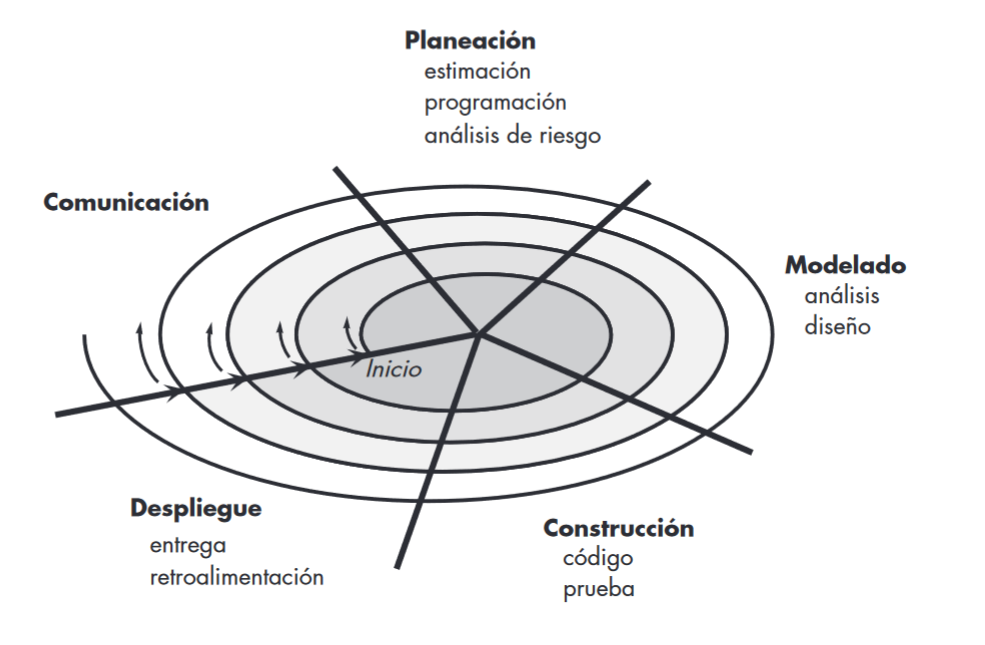
\includegraphics[width=\linewidth]{Figures/model-spiral.png}
	\caption{Modelo espiral. Fuente: \cite{pressman2010ingeneria}}
\end{figure}

Una característica clave del modelo espiral es su enfoque en la gestión de riesgos en cada ciclo. En cada paso del proceso, se realiza una evaluación de riesgos, lo que permite identificar y mitigar problemas potenciales antes de que se conviertan en obstáculos significativos. Este enfoque iterativo permite a los desarrolladores y clientes entender mejor y reaccionar a los riesgos en cada nivel de evolución del proyecto. Esta capacidad para adaptarse y evolucionar con el tiempo lo hace particularmente útil en entornos dinámicos y en constante cambio.

El desafío de este modelo radica en que requiere una evaluación continua y experta de los riesgos, y puede ser difícil convencer a los clientes, especialmente en situaciones contractuales, de que el enfoque iterativo y evolutivo es controlable y efectivo. Además, la complejidad en la gestión del proyecto puede aumentar debido a la necesidad de revisiones y ajustes continuos en cada ciclo.

\subsection{Metodología Scrum}

Scrum es una metodología ágil de desarrollo de software que se alinea con los principios del Manifiesto Ágil, promoviendo flexibilidad, colaboración continua, y adaptabilidad a los cambios. Este modelo estructura el desarrollo en ciclos cortos y repetitivos llamados sprints, típicamente de 2 semanas, donde no se permiten cambios durante el sprint, proporcionando estabilidad mientras se abordan los requisitos seleccionados del backlog, una lista dinámica y priorizada de tareas del proyecto que puede modificarse en cualquier momento \cite{pressman2010ingeneria}.

El proceso de Scrum incluye reuniones diarias breves donde cada miembro del equipo responde a tres preguntas fundamentales sobre sus avances, obstáculos, y planes, lo que ayuda a identificar y resolver problemas rápidamente, fomentando la autoorganización y eficiencia del equipo. Al final de cada sprint, se realiza una demostración al cliente del incremento de software desarrollado, facilitando la retroalimentación vital que influirá en los siguientes sprints y asegurando que el producto final cumpla con las expectativas del cliente.

\begin{figure}[h]
	\centering
	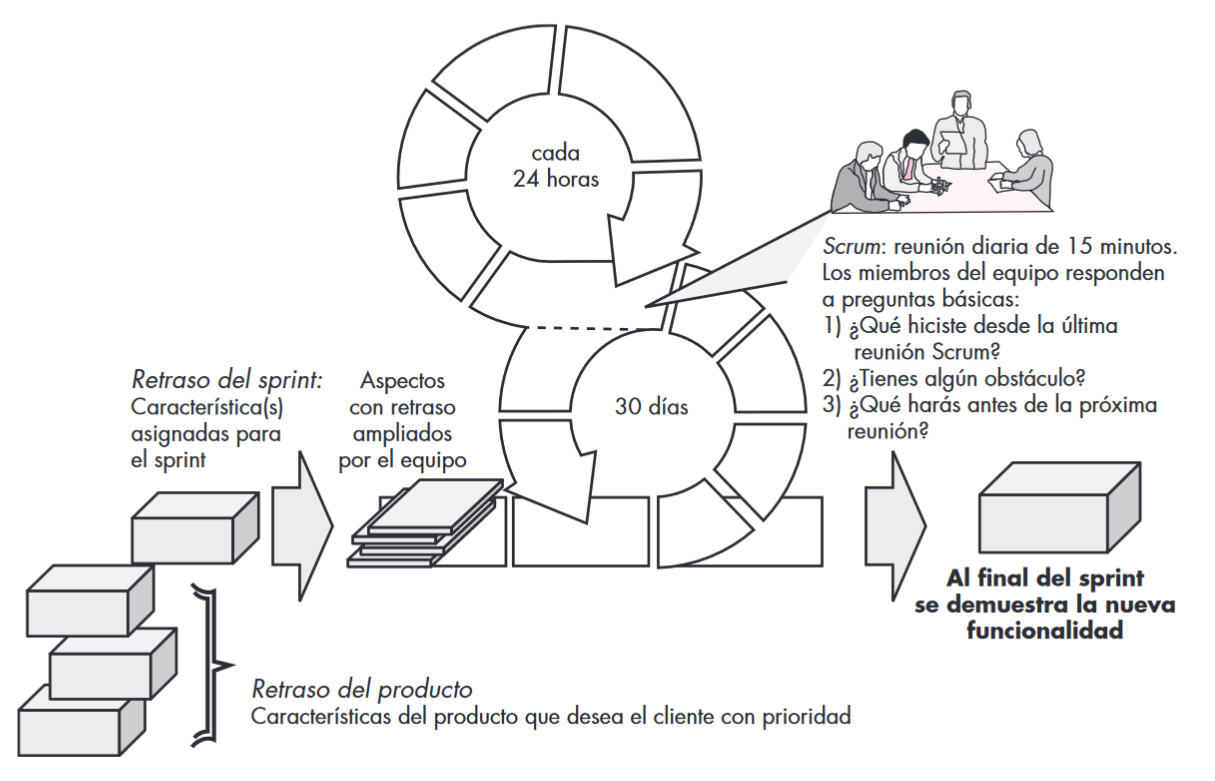
\includegraphics[width=\linewidth]{Figures/model-scrum.png}
	\caption{Metodología Scrum. Fuente: \cite{pressman2010ingeneria}}
\end{figure}

Scrum es efectivo en entornos donde la incertidumbre es la norma, aceptando el caos como una parte inherente del desarrollo de software y ofreciendo herramientas para gestionarlo de manera efectiva. La iteración continua, evaluación constante de riesgos, y la involucración directa del cliente permiten dirigir proyectos hacia resultados exitosos, incluso en circunstancias desafiantes, haciendo de Scrum una metodología ideal para proyectos que exigen flexibilidad y colaboración estrecha con el cliente.

\subsection{Metodología Kanban}

El método Kanban es un enfoque visual para la gestión del flujo de trabajo. Este método busca optimizar la eficiencia al evitar la sobrecarga de trabajo, eliminando cuellos de botella y desperdicios, y reduciendo los tiempos de espera, lo que a su vez incrementa el rendimiento de los procesos \cite{alaidaros2021kanban}.

Kanban se centra en la utilización de un sistema de "pull" (extracción), donde el trabajo solo se inicia cuando hay capacidad disponible, lo que permite una mayor adaptabilidad y respuesta a los cambios en las prioridades del proyecto. Este enfoque se visualiza mediante el tablero Kanban, dividido en columnas que representan diferentes etapas del proceso de desarrollo. Cada tarea o 'tarjeta' se mueve de izquierda a derecha a través del tablero, reflejando su progreso desde el inicio hasta la finalización. Las columnas básicas de un tablero Kanban incluyen "Por hacer", "En progreso" y "Completado", aunque el tablero puede personalizarse agregando columnas adicionales según las necesidades del proyecto.

\begin{figure}[h]
	\centering
	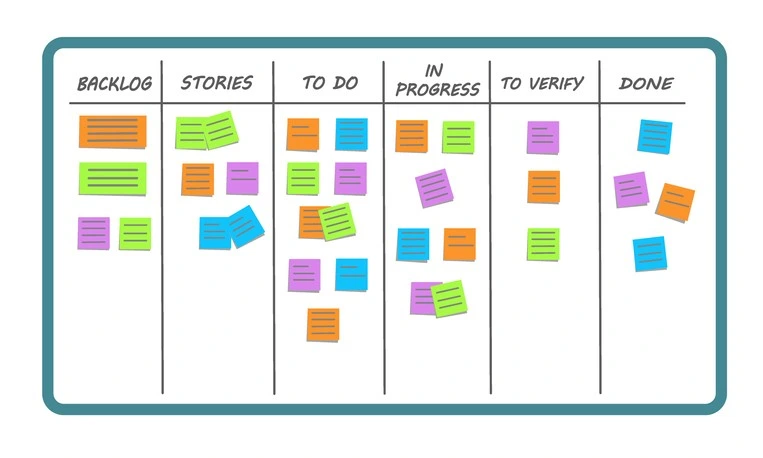
\includegraphics[width=\linewidth]{Figures/model-kanban.png}
	\caption{Tablero Kanban de ejemplo.}
\end{figure}

Este método define cinco principios claves para la práctica: limitar el trabajo en progreso, visualizar el flujo de trabajo, medir y gestionar el flujo, hacer explícitas las políticas del proceso, y utilizar modelos para reconocer oportunidades de mejora. Estos principios ayudan a mantener el enfoque en la eficiencia del flujo de trabajo y en la mejora continua, permitiendo al equipo adaptar sus prácticas y procesos según las necesidades del proyecto y las condiciones del entorno.

Kanban no requiere cambios estructurales grandes para su implementación y se adapta a la situación actual de cualquier organización. Una posible desventaja es que Kanban requiere una disciplina rigurosa y una comunicación constante dentro del equipo para mantener la precisión del flujo visualizado en el tablero y que se corresponda con la realidad, lo que puede ser desafiante en equipos grandes. Además, la falta de fases definidas y la ausencia de revisiones sistemáticas del progreso pueden dificultar la gestión de proyectos a gran escala, donde se requiere una coordinación extensa entre múltiples equipos o disciplinas. A su vez, Kanban puede no ser adecuado para proyectos que enfrentan cambios frecuentes y radicales en los requerimientos, ya que está diseñado para optimizar flujos de trabajo existentes más que para adaptarse a innovaciones constantes.

\section{Comparación de metodologías}

A continuación, se presenta a modo de resumen una comparación de las metodologías de desarrollo de software analizadas en distintos aspectos clave para determinar cuál es la más adecuada para el desarrollo de software de este trabajo de tesis.

\section{Ágil (Scrum)}
\begin{itemize}
    \item \textbf{Naturaleza del Proyecto}: Ideal para proyectos con requisitos cambiantes y evolución constante.
    \item \textbf{Requisitos del Cliente}: Los requisitos pueden cambiar en cada sprint, permitiendo interacción continua con el cliente.
    \item \textbf{Tamaño del Equipo}: Equipos pequeños (idealmente 5-9 personas), colaborativos y multidisciplinarios.
    \item \textbf{Cultura Organizacional}: Cultura colaborativa, centrada en la mejora continua y la autoorganización.
    \item \textbf{Flexibilidad en Gestión}: Alta flexibilidad para adaptarse a los cambios durante cada sprint (iteración).
    \item \textbf{Documentación}: Documentación mínima, suficiente para facilitar la entrega de valor funcional.
    \item \textbf{Riesgos y Control de Calidad}: Los riesgos se manejan en cada sprint, con pruebas y ajustes continuos.
    \item \textbf{Entregas al Cliente}: Entregas frecuentes (cada sprint), con incrementos de software funcional.
    \item \textbf{Curva de Aprendizaje}: Media. Requiere adaptación a la metodología y roles dentro del equipo.
    \item \textbf{Velocidad de Desarrollo}: Alta. Las iteraciones cortas permiten entregas rápidas y ajustes según la retroalimentación.
    \item \textbf{Manejo de Cambios}: Cambios fáciles de gestionar en cada sprint.
    \item \textbf{Manejo de Riesgos}: Riesgos gestionados en cada sprint, con retrospectivas que permiten mejoras continuas.
\end{itemize}

\section{Ágil (Kanban)}
\begin{itemize}
    \item \textbf{Naturaleza del Proyecto}: Proyectos que requieren flujo continuo y flexibilidad para gestionar tareas.
    \item \textbf{Requisitos del Cliente}: Los requisitos pueden ajustarse de manera continua según la demanda y prioridades.
    \item \textbf{Tamaño del Equipo}: Equipos pequeños a medianos, más flexibles en tamaño, ajustando tareas según el flujo de trabajo.
    \item \textbf{Cultura Organizacional}: Cultura flexible y adaptable, con enfoque en la optimización del flujo de trabajo.
    \item \textbf{Flexibilidad en Gestión}: Alta flexibilidad en la gestión del flujo, ajustando la carga de trabajo en función de prioridades.
    \item \textbf{Documentación}: Documentación mínima, enfocada en la visualización del flujo y el progreso.
    \item \textbf{Riesgos y Control de Calidad}: Control continuo del flujo de trabajo, evitando cuellos de botella.
    \item \textbf{Entregas al Cliente}: Entregas continuas, en función de la finalización de tareas o según demanda.
    \item \textbf{Curva de Aprendizaje}: Baja. Fácil de implementar, basado en la mejora continua del flujo de trabajo.
    \item \textbf{Velocidad de Desarrollo}: Alta. Flujo continuo de desarrollo, ajustando la velocidad según prioridades.
    \item \textbf{Manejo de Cambios}: Los cambios se gestionan en función de la demanda, ajustando tareas en el flujo de trabajo.
    \item \textbf{Manejo de Riesgos}: Riesgos manejados de manera continua, ajustando el flujo y reduciendo cuellos de botella.
\end{itemize}

\section{Cascada}
\begin{itemize}
    \item \textbf{Naturaleza del Proyecto}: Adecuado para proyectos con requisitos claros y definidos desde el principio.
    \item \textbf{Requisitos del Cliente}: Requisitos fijos desde el inicio, cualquier cambio implica un costo significativo.
    \item \textbf{Tamaño del Equipo}: Equipos medianos a grandes, con roles bien definidos y fases claras.
    \item \textbf{Cultura Organizacional}: Cultura jerárquica y estructurada, con fases bien definidas.
    \item \textbf{Flexibilidad en Gestión}: Baja flexibilidad, difícil de cambiar una vez iniciado el proyecto.
    \item \textbf{Documentación}: Documentación detallada en cada fase del ciclo de vida del desarrollo.
    \item \textbf{Riesgos y Control de Calidad}: Riesgo alto si los requisitos cambian, control de calidad al final del ciclo.
    \item \textbf{Entregas al Cliente}: Una única entrega al final del proyecto.
    \item \textbf{Curva de Aprendizaje}: Baja. Fácil de comprender, pero difícil de ajustar a cambios durante el ciclo.
    \item \textbf{Velocidad de Desarrollo}: Baja a media. El ciclo es largo debido a la rigidez en las fases.
    \item \textbf{Manejo de Cambios}: Cambios difíciles y costosos de implementar una vez que el proyecto ha avanzado.
    \item \textbf{Manejo de Riesgos}: Riesgo alto, ya que los problemas suelen descubrirse al final, durante la fase de prueba.
\end{itemize}

\section{Modelo en V}
\begin{itemize}
    \item \textbf{Naturaleza del Proyecto}: Proyectos de alta criticidad, con un enfoque riguroso en calidad y validación.
    \item \textbf{Requisitos del Cliente}: Requisitos claros desde el inicio, con verificación constante.
    \item \textbf{Tamaño del Equipo}: Equipos medianos a grandes, con roles especializados para cada fase.
    \item \textbf{Cultura Organizacional}: Cultura disciplinada y centrada en la calidad, con un fuerte enfoque en la validación y verificación.
    \item \textbf{Flexibilidad en Gestión}: Flexibilidad moderada, cambios difíciles una vez avanzado el proyecto.
    \item \textbf{Documentación}: Documentación extensa, especialmente en fases de pruebas y validación.
    \item \textbf{Riesgos y Control de Calidad}: Riesgo bajo, con verificación y validación constante en cada fase.
    \item \textbf{Entregas al Cliente}: Una única entrega al final, con validación en cada fase.
    \item \textbf{Curva de Aprendizaje}: Media. Se requiere disciplina en verificación y validación.
    \item \textbf{Velocidad de Desarrollo}: Media. Las fases de validación pueden ralentizar el desarrollo.
    \item \textbf{Manejo de Cambios}: Los cambios son complicados, requieren revalidación constante.
    \item \textbf{Manejo de Riesgos}: Riesgo bajo, debido a la verificación y validación constantes en cada fase.
\end{itemize}

\section{Espiral}
\begin{itemize}
    \item \textbf{Naturaleza del Proyecto}: Proyectos grandes y complejos, con alto riesgo y múltiples iteraciones.
    \item \textbf{Requisitos del Cliente}: Los requisitos pueden refinarse en cada iteración, ideal para proyectos con incertidumbre.
    \item \textbf{Tamaño del Equipo}: Equipos medianos a grandes, flexibles en roles según los ciclos de iteración y gestión de riesgos.
    \item \textbf{Cultura Organizacional}: Cultura orientada a la gestión del riesgo y adaptación a cambios continuos en cada iteración.
    \item \textbf{Flexibilidad en Gestión}: Alta flexibilidad, con ciclos iterativos que permiten gestionar cambios de forma continua.
    \item \textbf{Documentación}: Documentación formal en cada iteración para gestionar riesgos y validar avances.
    \item \textbf{Riesgos y Control de Calidad}: Riesgo bajo, diseñado específicamente para gestionar riesgos en cada iteración.
    \item \textbf{Entregas al Cliente}: Entregas iterativas, con revisiones parciales hasta completar el proyecto.
    \item \textbf{Curva de Aprendizaje}: Alta. Complejidad en la gestión del riesgo y las iteraciones continuas.
    \item \textbf{Velocidad de Desarrollo}: Media. El proceso iterativo es más largo por la gestión de riesgos y planificación.
    \item \textbf{Manejo de Cambios}: Cambios gestionados de manera continua en cada ciclo, permitiendo ajustes según los riesgos.
    \item \textbf{Manejo de Riesgos}: Riesgo bajo, diseñado para gestionar riesgos en cada iteración de manera efectiva.
\end{itemize}


\section{Selección de metodología}

En base al análisis realizado, elegimos el modelo en V y Kanban como las metodologías más adecuadas, para el desarrollo de este proyecto de tesis, debido a sus características y beneficios particulares que se alinean con los requisitos y condiciones del proyecto.

En el proceso de elección de metodología, comenzamos prescindiendo el uso de las metodologías que no se ajustaban a las necesidades y características del proyecto. Luego, comparamos las metodologías restantes en función de los aspectos clave mencionados anteriormente, para determinar cuál se ajusta mejor a los objetivos y condiciones del proyecto.

En el proceso de selección de metodologías para este proyecto, en primer lugar, se desestimó el uso Scrum por varias razones específicas. Scrum, aunque es potente en proyectos que requieren flexibilidad y adaptación continua, fue filtrado principalmente porque necesita una presencia activa y constante del cliente o un Product Owner para guiar los sprints, lo cual no es posible en este proyecto. Además, la estructura de equipo pequeño y la falta de roles específicos como Scrum Master y Product Owner complican la implementación de Scrum, que además implica reuniones regulares intensivas que no se alinean con la capacidad del equipo, ya que cobran mayor sentido en proyectos con equipos más grandes con mayor diversidad de roles y responsabilidades con necesidad de sincronización frecuente.

Por otro lado, la metodología en espiral, que se centra en la gestión de riesgos y adaptación a cambios continuos, fue considerada innecesariamente compleja para este proyecto dado que los riesgos y la incertidumbre son relativamente bajos y no justifican el tiempo adicional y la complejidad que esta metodología implicaría. Por estos motivos, se desestimó la metodología en espiral en favor de enfoques más simples y directos.

En base al análisis realizado sobre las metologías restantes, elegimos el modelo en V y Kanban como las metodologías más adecuadas para el desarrollo de este proyecto de tesis, debido a sus características y beneficios particulares que se alinean con los requisitos y condiciones del proyecto. El modelo en V se seleccionó sobre el modelo en cascada aunque ambos son aplicables a equipos de cualquier tamaño y proyectos de cualquier envergadura. Ambos modelos se centran en la planificación y la documentación, lo cual es apropiado para este proyecto dado que los requerimientos están claramente definidos y la probabilidad de cambios y de riesgo es baja, gracias a una investigación y análisis exhaustivos realizados previamente.

El modelo en V ofrece la ventaja de validar y verificar cada módulo de software funcional antes de avanzar a la siguiente fase, permitiendo correcciones tempranas en caso de errores o cambios, lo que aumenta la flexibilidad y adaptabilidad del proyecto. Este enfoque de validación continua en cada fase contrasta con el modelo en cascada, que, aunque estructurado, avanza secuencialmente sin permitir el retroceso, lo que puede complicar la corrección de errores detectados en fases tardías. Por lo tanto, el modelo en V es preferido por su capacidad para manejar mejor el riesgo y por ofrecer una estructura que facilita la adaptación y mejora continua del proyecto.

Para este trabajo, este sistema de validación y verificación constante es especialmente valioso, ya que el sistema incluye un componente crítico, como lo es el contrato inteligente de trazabilidad en blockchain, que una vez desplegado, no puede ser actualizado para corregir errores, modificar comportamientos o añadir nuevas funcionalidades. Por lo tanto, es crucial que cada fase del desarrollo sea validada y verificada rigurosamente para garantizar la calidad y la integridad del sistema final antes de su despeliegue.

Adicionalmente, se decidió integrar Kanban para la gestión de tareas y el seguimiento del flujo de trabajo durante el desarrollo. Kanban complementará al modelo en V al proporcionar una mayor flexibilidad en la gestión de micro-tareas y prioridades diarias, sin sobrecargar al pequeño equipo de trabajo. Esta metodología es ligera y fácil de implementar, y su naturaleza visual ayuda a mantener una vista clara del avance del proyecto, facilitando el seguimiento y la intervención rápida por parte del tutor y el estudiante.

La combinación de estas dos metodologías permitirá al equipo de trabajo mantener un equilibrio entre la rigurosidad y la flexibilidad, garantizando la calidad y la validación en cada fase del proyecto, mientras se mantiene la adaptabilidad y la eficiencia en la gestión de tareas diarias.

\subsection{Implementación Conjunta de Metodologías}

La implementación conjunta del modelo en V y Kanban será llevada a cabo utilizando un enfoque integrado que capitaliza las fortalezas de ambas metodologías. El modelo en V guiará la estructura general del proceso de desarrollo, asegurando que cada etapa del proyecto, desde la planificación hasta la validación, se ejecute con un enfoque en la calidad y la documentación rigurosa. Paralelamente, Kanban se aplicará dentro de cada etapa del modelo en V para gestionar y visualizar las tareas diarias. Esto permitirá controlar el progreso y hacer ajustes operativos sin comprometer la estructura metodológica del modelo en V. El uso de un tablero Kanban facilitará la visualización del estado de las tareas en tiempo real, promoviendo una gestión ágil que se ajusta a la dinámica del equipo y los requerimientos del proyecto.

La combinación de estas metodologías asegura un balance entre la rigurosidad y la flexibilidad dentro del proceso de desarrollo, permitiendo que el equipo mantenga una planificación clara y una gestión eficiente de tareas, al mismo tiempo que se enfoca en una entrega final de alta calidad y bien documentado.

